% !TEX root = ../main.tex

\chapter{Data processing}
\label{ch:data_processing}




\section{Processing flow}

Schema Datasets -> xxx\_preprocessing.py -> create\_dataset.py -> Train/Val


\subsection{PROSTATEx: From DICOM to NumPy arrays}

The PROSTATEx dataset comes with two CSV files for the training set. The first one, \textit{ProstateX-Findings-Train.csv}, lists all findings with their clinical significance. Multiple findings can be associated with the same patient (ProxID). The second one, \textit{ProstateX-Images-Train.csv}, gives information about where to find the right DICOM file for each patient and each finding. Important labels are "ProxID" (patient ID), "fid" (finding ID, from 1 to $\infty$), "ClinSig" (clinical significance, TRUE or FALSE), "DCMSerNumber" (digit before the dash in the folder name containing DICOM files) and "ijk" (position of the lesion: slice number $k$ at coordinates $(i,j)$, $i,j,k \in [0,\infty]$). Both CSV files are complementary to each other. Algorithm \ref{alg:PROSTATEx_preprocessing} describes the steps involved in converting PROSTATEx's DICOM files to NumPy arrays. 

\begin{algorithm}
    \caption{PROSTATEx preprocessing}
    \label{alg:PROSTATEx_preprocessing}
    \begin{algorithmic}[1] % The number tells where the line numbering should start
        \Procedure{main}{$dataset\_folder, findings\_CSV, slices\_CSV, output\_folder$}
        		\State Create output directories: $"output\_folder/True", "output\_folder/False"$\\
        		\State $findings \gets read\_CSV(findings\_CSV)$ \Comment{ProstateX-Findings-Train.csv}
        		\State $slices \gets read\_CSV(slices\_CSV)$ \Comment{ProstateX-Images-Train.csv}
            \State $meta \gets merge(findings, slices)$\Comment{Both CSV files are complementary to each other.}\\
            \For{$row$ in $meta$}
            		\State $patient\_id \gets row["ProxID"]$
            		\State $finding\_id \gets row["fid"]$
            		\State $mri\_type\_number \gets row["DCMSerNumber"]$
            		\State $clinical\_significance \gets row["ClinSig"]$
            		\State $img\_i, img\_j, img\_k \gets row["ijk"]$
            		\State $slice\_number \gets img\_k + 1$ \Comment{CSV indexing in $[0,\infty]$, DICOM in $[1,\infty]$}\\
                \For{$visit\ in\ patient\_id$'s folder}
                		\For{$mri\_type$ in $visit$}
                			\If {$mri\_type$ starts with "$mri\_type\_number$-"}
                				\For{$dicom\_file$ in $mri\_type$}
                					\If {$slice\_number == dicom\_file.InstanceNumber$}
                						\State{$slice \gets normalize\_dicom(dicom\_file)$} \Comment{see section \ref{sec:dicom_data_manipulation}}
                						\State{Save $slice$ in $"output\_folder/clinical\_significance"$}
                					\EndIf
                				\EndFor
                			\EndIf
            			\EndFor
            		\EndFor
            \EndFor
        \EndProcedure
    \end{algorithmic}
\end{algorithm}



\subsection{Lung CT Challenge - From DICOM to NumPy arrays}

Lung CT Challenge is composed of two different subdatasets: one is considered as a calibration set (10 patients) and the other as a test set (60 patients). Since labels were provided for both sets and the amount of data is fairly low, they were merged and used as a training set. 

Regarding labelling, two Excel files, \textit{TestSet\_NoduleData\_PublicRelease\_wTruth} and \textit{CalibrationSet\_NoduleData}, contain labels for these images. In order to facilitate label managing, two CSV files were manually created: \textit{TestSet.csv} and \textit{CalibrationSet.csv}.
Contrary to PROSTATEx, more than two labels were used for this dataset. Both "malignant" and "Primary lung cancer" were considered as positive, whereas "benign" and "Benign nodule" as negative. A third label called "Suspicious malignant nodule" appeared two times. Since the diagnosis was not clearly defined for those images, they were not treated and included in the training data in order to avoid any noise. Algorithm \ref{alg:LungCTChallenge_preprocessing} shows the various processing steps.

\begin{algorithm}
    \caption{Lung CT Challenge preprocessing}
    \label{alg:LungCTChallenge_preprocessing}
    \begin{algorithmic}[1] % The number tells where the line numbering should start
        \Procedure{main}{$dataset\_folder, train\_CSV, test\_CSV, output\_folder$}
        		\State Create output directories: $"output\_folder/True", "output\_folder/False"$\\
        		\State $csv\_training \gets read\_CSV(train\_CSV)$ \Comment{CalibrationSet.csv}
        		\State $csv\_test \gets read\_CSV(test\_CSV)$ \Comment{TestSet.csv}
            \State $csv\_concatenated \gets concat(csv\_training, csv\_test)$\Comment{Both CSV files contain similar information about different patients.}\\
            \For{$row$ in $csv\_concatenated$}
            		\State $patient\_id \gets row["Scan\ Number"]$
            		\State $slice\_number \gets row["Nodule\ Center\ Image"]$ \Comment{Value in $[1,\infty]$}
            		\State $finding\_id \gets row["Nodule\ Number"]$
            		\State $clinical\_significance \gets row["Diagnosis"]$\\
            		\If{$clinical\_significance$ == $"malignant"$ or $"Primary\ lung\ cancer"$}
            			\State{$clinical\_significance \gets True$}
            		\ElsIf{$clinical\_significance$ == $"benign"$ or $"Benign\ nodule"$}
            			\State{$clinical\_significance \gets False$}
            		\ElsIf {$"clinical\_significance$ == $"Suspicious\ malignant\ nodule"$}
            			\State{Continue}
            		\EndIf\\
                \For{$visit\ in\ patient\_id$'s folder}
                		\For{$mri\_type$ in $visit$}
                			\For{$dicom\_file$ in $mri\_type$}
                				\If {$slice\_number == dicom\_file.InstanceNumber$}
                					\State{$slice \gets normalize\_dicom(dicom\_file)$} \Comment{see section \ref{sec:dicom_data_manipulation}}
                					\State{Save $slice$ in $"output\_folder/clinical\_significance"$}
                				\EndIf
                			\EndFor
            			\EndFor
            		\EndFor
            \EndFor
        \EndProcedure
    \end{algorithmic}
\end{algorithm}


\subsection{NumPy arrays to PNG files}
Exporting to NumPy arrays instead of image files directly has multiple advantages. First of all, converting medical files to NumPy arrays or PNG files takes more time than converting NumPy arrays to image files. Reason for that is that the former requires a lot of operation as well as pixel normalization, whereas the latter is a mere conversion of one format to the other. This makes data more reusable. Then, it facilitates the debugging process by separating the conversion from medical files to PNG files into two different steps. Finally, the same processing script can be used to convert NumPy arrays from any dataset to PNG images, which eases operations such as generating different training-validation splits, augmenting data, etc.

\begin{algorithm}
    \caption{Create dataset - NumPy arrays to PNG conversion, organizing data into training and validation data}
    \label{alg:create_dataset}
    \begin{algorithmic}[1] % The number tells where the line numbering should start
        \Procedure{create\_pngs}{$dataset\_folder, output\_folder, split$}
        		\State Create output directories: $"output\_folder/[Train|Val]/[0|1]"$\\
        		\State $true\_nparrays\_dict \gets \{"patient\_id" : [file\_name\_1, ...]\}$
        		\State $number\_of\_patients\_true \gets len(true\_nparrays\_dict)$
        		\State $number\_of\_training\_patients\_true \gets \lfloor number\_of\_patients\_true * split \rfloor$
        		\State $false\_nparrays\_dict \gets \{"patient\_id" : [file\_name\_1, ...]\}$\\
        		\State $index \gets 0$
        		\For{$patient\_id, file\_names$ in $true\_nparrays\_dict$}
        			\If{$index < number\_of\_training\_patients\_true$} \Comment{Training set, True}
        				\For{$file\_name$ in $file\_names$}
        					\State $image\_array \gets load(file\_name)$
        					\State $image \gets convertArrayToGrayscaleImage(image\_array)$
        					\State Save image to $"output\_folder/Train/1"$
        				\EndFor
        			\Else \Comment{Validation set, True}
        				\For{$file\_name$ in $file\_names$}
        					\State $image\_array \gets load(file\_name)$
        					\State $image \gets convertArrayToGrayscaleImage(image\_array)$
        					\State Save image to $"output\_folder/Val/1"$
        				\EndFor
        			\EndIf
        			\State{$index \gets index + 1$}
        		\EndFor\\
        		\State $number\_of\_training\_patients\_false \gets \lfloor number\_of\_patients\_false * split \rfloor$
        		\State $false\_nparrays\_dict \gets \{"patient\_id" : [file\_name\_1, ...]\}$
        		\State $number\_of\_patients\_false \gets len(false\_nparrays\_dict)$
        		\State $false\_nparrays\_dict \gets \{"patient\_id" : [file\_name\_1, ...]\}$\\
        		\State $index \gets 0$
        		\For{$patient\_id, file\_names$ in $false\_nparrays\_dict$}
        			\If{$index < number\_of\_training\_patients\_false$} \Comment{Training set, False}
        				\For{$file\_name$ in $file\_names$}
        					\State $image\_array \gets load(file\_name)$
        					\State $image \gets convertArrayToGrayscaleImage(image\_array)$
        					\State Save image to $"output\_folder/Train/0"$
        				\EndFor
        			\Else \Comment{Validation set, False}
        				\For{$file\_name$ in $file\_names$}
        					\State $image\_array \gets load(file\_name)$
        					\State $image \gets convertArrayToGrayscaleImage(image\_array)$
        					\State Save image to $"output\_folder/Val/0"$
        				\EndFor
        			\EndIf
        			\State{$index \gets index + 1$}
        		\EndFor
        \EndProcedure
    \end{algorithmic}
\end{algorithm}

Algorithm \ref{alg:create_dataset} describes how data was split and organized in order for PyTorch to make use of it. To do so, they were split by class (True $\equiv$ 1, False $\equiv$ 0) and role (training or validation). Furthermore, data are split by patients and not by slices. In fact, multiple slices are usually assigned to each patient. Instead of considering each slice separately, which allows to divide a single patient's slices into the training and validation folders, they were treated as a whole. To sum up, an 80-20 split between the training and validation data (split argument set to $0.8$) will use 80\% of the patients as training data and 20\% of the patients as validation data, regardless of the number of slices.


\subsection{Data augmentation}

The amount of publicly available data is relatively limited. However, deep learning models require a lot of training data to be able to learn and generalize well. Therefore, augmenting data allows to create more training examples from the ones available. To achieve this, multiple techniques such as rotation, flipping, cropping and shifting can be used. Algorithm \ref{alg:augment} describes how data was augmented. Given an MR image, a large patch centered on the lesion was cropped first, which makes the rotation process easier. In fact, rotating the image without cropping it first also moves the region of interest. In this case, finding the exact coordinates becomes more complicated. Therefore, a first large patch was created and then rotated. Afterwards, a smaller patch around the region of interest was extracted because of the potential padding induced by the rotation. This guarantees the addition of the minimal amount of padding pixels around the image to plug the holes, which decreases the probability of adding artificial information to the image.

\begin{algorithm}
    \caption{Create augmented dataset - Augmentation method}
    \label{alg:augment}
    \begin{algorithmic}[1] % The number tells where the line numbering should start
        \Procedure{augment}{$image, img\_i, img\_j, available\_combinations\_list$}
        		%\Comment{image: Pillow image, img\_[i,j]: position of the lesion, available\_combinations\_list: tuples (degree, prob\_flipping)}\\
        		\State{$index \gets$ random index in $[0, $len(available\_combinations\_list)$ - 1]$}
        		\State{$degree, prob\_flipping = available\_combinations\_list[index]$}
        		\State{Delete element $available\_combinations\_list[index]$} \Comment{Avoid duplication}\\
        		\State{$temp\_image \gets$ $image$.crop(64x64, center=$(img\_i, img\_j)$)} \Comment{$1^{st}$ crop}
        		\State{$temp\_image \gets\ temp\_image$.rotate(degree)} \Comment{Rotate $1^{st}$ crop}\\
        		\State{$width, height \gets$ $temp\_image$.size}
        		\State{$x\_center \gets \lfloor \frac{width}{2} \rfloor, y\_center \gets \lfloor \frac{height}{2} \rfloor$}\Comment{Find center pixel of $1^{st}$ crop}
        		\State{$temp\_image \gets$ $image$.crop(32x32, center=$(x\_center, y\_center)$)}\Comment{$2^{nd}$ crop}\\
        		\If{$prob\_flipping > 0.5$}
        			\State{$temp\_image \gets temp\_image.horizontal\_flip()$}
        		\EndIf\\
        		\Return $temp\_image$
        \EndProcedure
    \end{algorithmic}
\end{algorithm}


\subsection{Data visualization and verification}

Processing data manually increases the probability of making mistakes. For that matter, visualization tools relying on the same processing code as the ones used to generate training images were developped. Their goal was to compare our visual representation of an image to the one obtained in professional pieces of software. Also, PNG conversion was meticulously tested by comparing the pixel values from the original NumPy arrays with the PNG pixel values. 


\subsubsection{DICOM}

Visualizing DICOM files is pretty straightforward since each file represent a single two-dimensional image. However, the way this standard works require a lot of pixel transformation and normalization to obtain the desired result (see section \ref{sec:dicom_data_manipulation}), which may cause errors. Our tools allows to display a single DICOM file as well as a sequence of files if the function is feeded with a directory. Users can then scroll through the Z-axis, displaying the next or previous slice. 

\begin{figure}[!h]
\centering
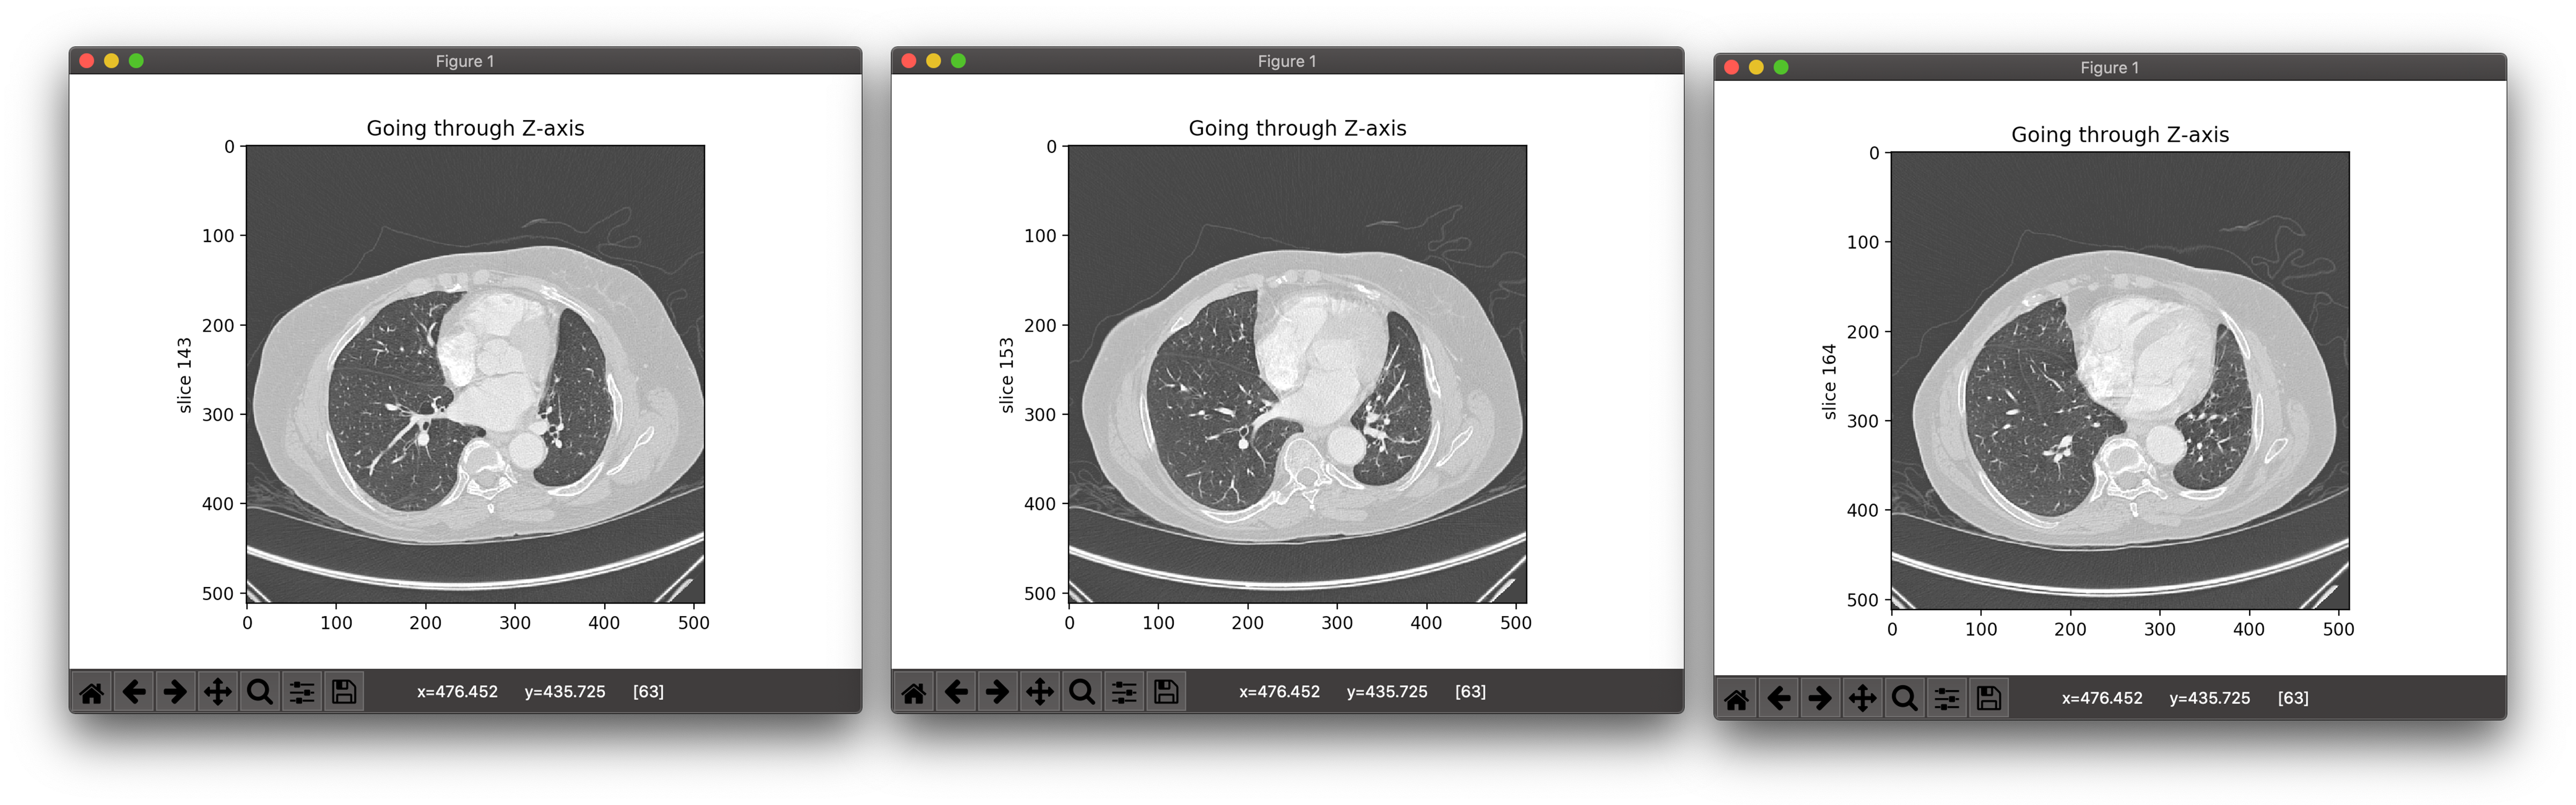
\includegraphics[width=\textwidth, keepaspectratio=true]{./figures/visualize_lung_dcm.png}
\caption{Visualization of a folder of DICOM files}
\label{fig:visualize_lung_dcm}
\end{figure}


\subsubsection{NIfTI}

As NIfTI files can be three or four-dimensional (the fourth dimension being time), our visualization tool takes this aspect into consideration by allowing to scroll through them: scrolling with the mouse goes through slices belonging to a specific timestamp over a specific axis, while the left and right arrows allows to jump to the corresponding slice with respect to another timestamp. When reaching the end of a timestamp with the mouse, the first slice of the next timestamp is displayed. Furthermore, the three-dimensionality implies that the volume is viewable under three different perspectives. For example, a three-dimensional brain volume can display it from the top of the head to the bottom, from one ear to the other and from the back of the head to the person's face. Therefore, the user can choose a specific axis to navigate through. If no axis is chosen, all three perspectives are shown one after the other.

\begin{figure}[!h]
\centering
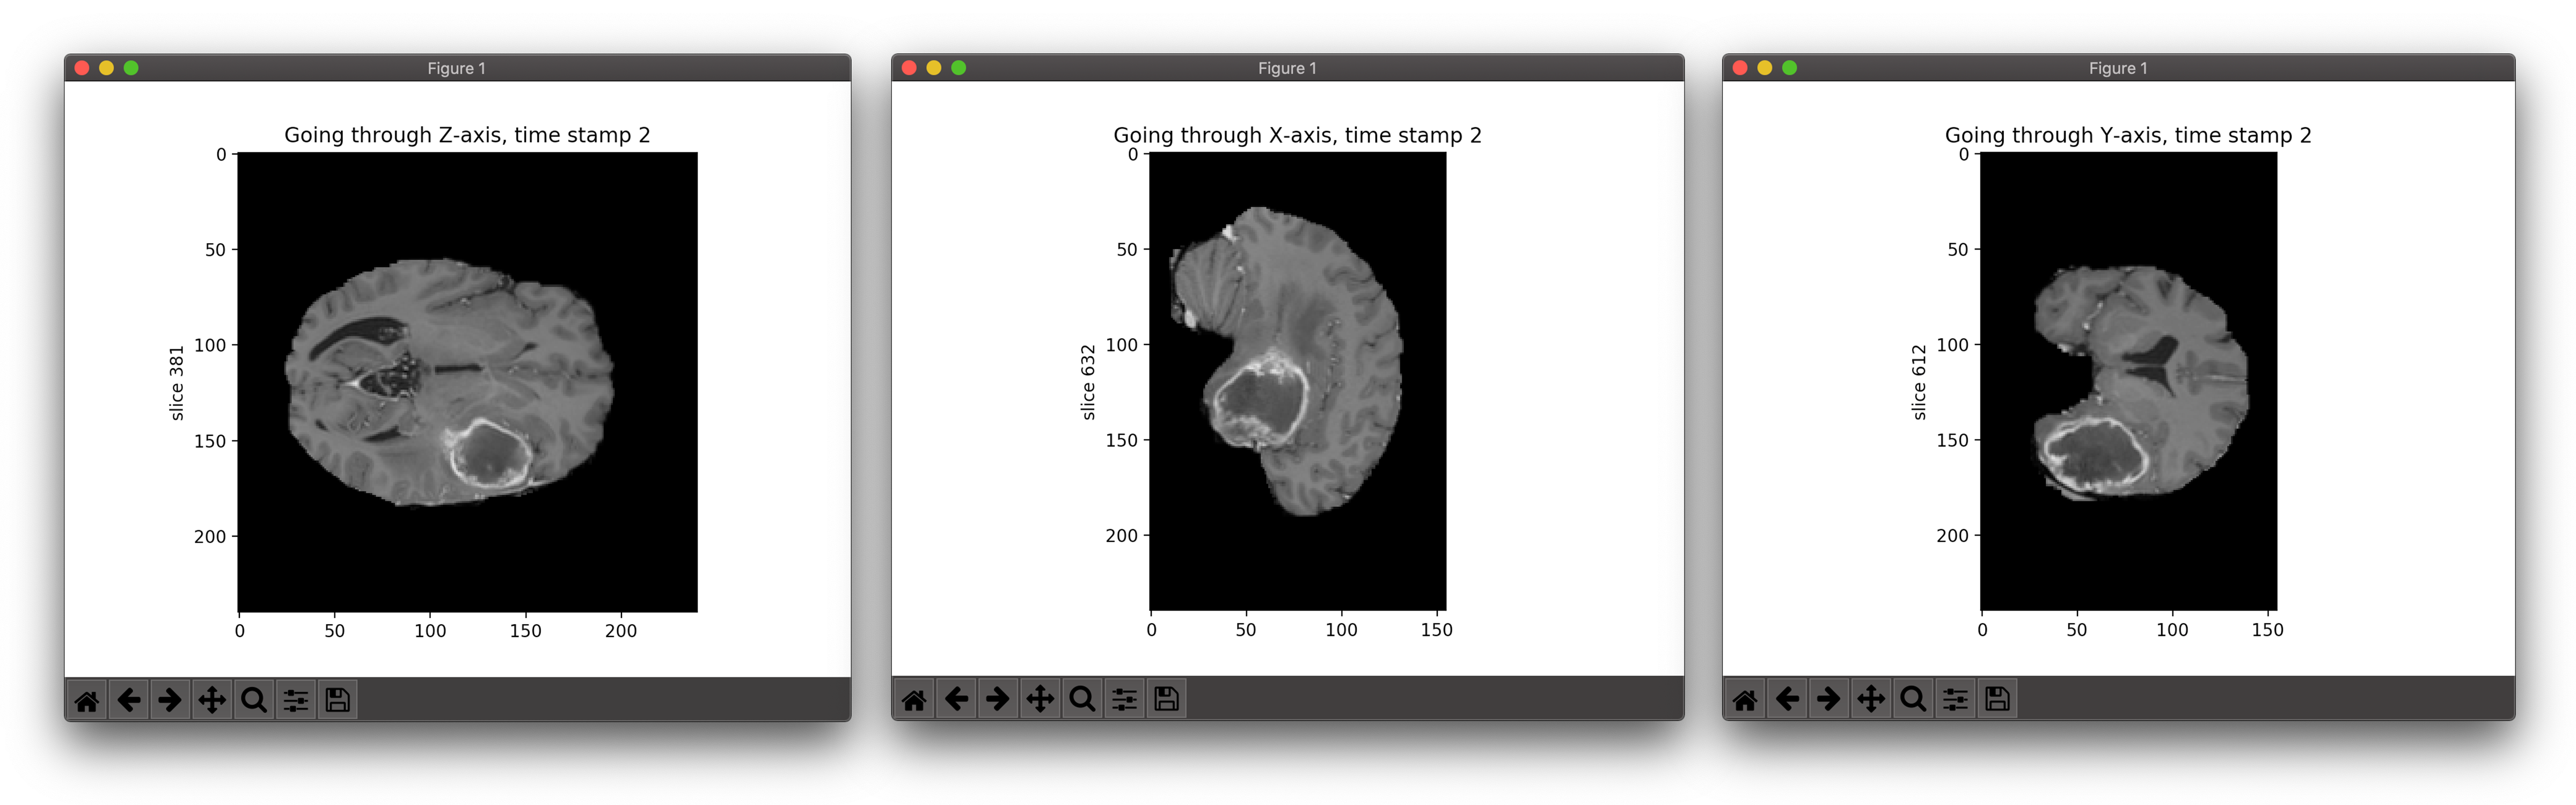
\includegraphics[width=\textwidth, keepaspectratio=true]{./figures/visualize_brain_nii.png}
\caption{Four-dimensional NIfTI visualization}
\label{fig:visualize_brain_nii}
\end{figure}



\subsubsection{RAW}

Medical RAW files are three-dimensional. Scrolling with the mouse goes through slices over a specific axis. Like NIfTI, the user can profit from the three-dimensionality by navigating through slices under three different perspectives.

\begin{figure}[!h]
\centering
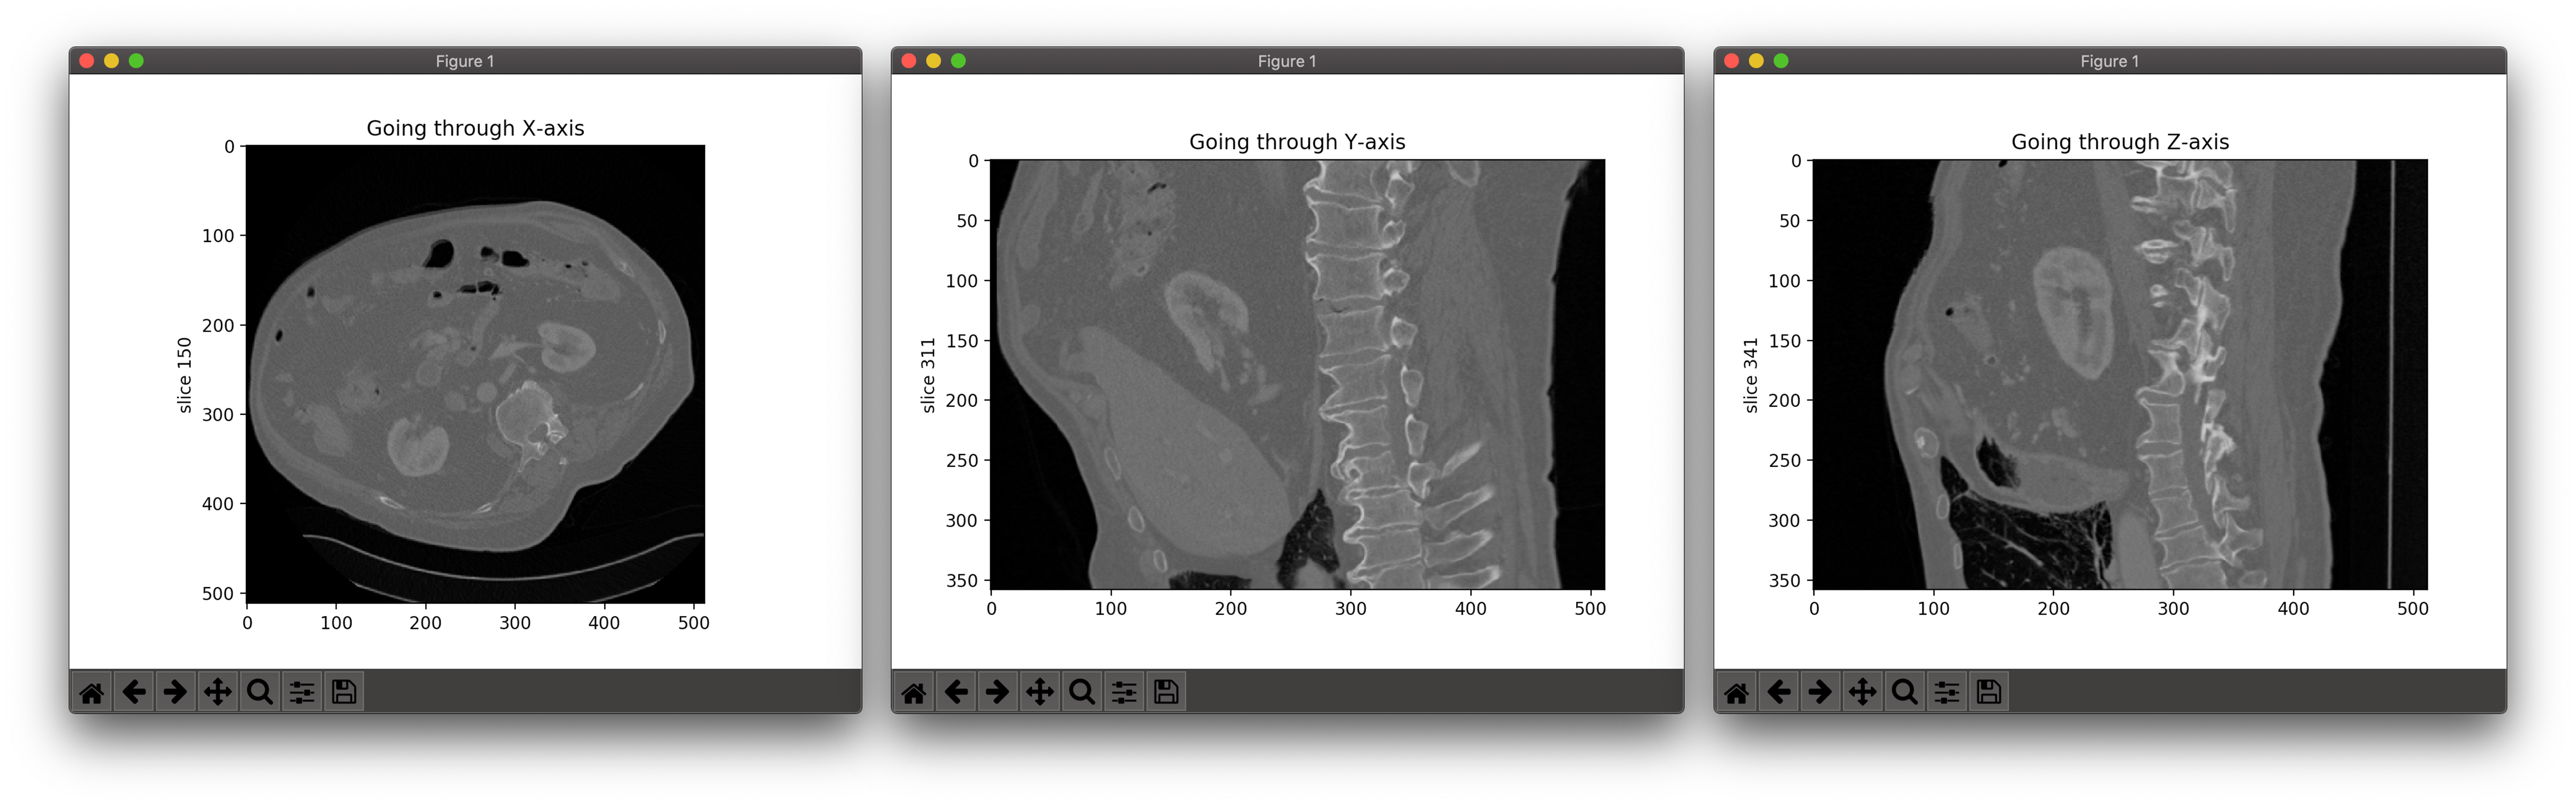
\includegraphics[width=\textwidth, keepaspectratio=true]{./figures/visualize_liver_raw.png}
\caption{Three-dimensional RAW visualization}
\label{fig:visualize_liver_raw}
\end{figure}

